%%%%%%%%%%%%%%%%%%%%%%%%%%%%%%%%%%%%%%%%%%%%%%%%%%%%%%%%%%%%%%%%%%%%%%%%%%%%%%%%%%%%%%%%%%%%%%%%%%%%%%%%%%%%%%%%%%%%%%%%%
\subsection{Intuition}
%%%%%%%%%%%%%%%%%%%%%%%%%%%%%%%%%%%%%%%%%%%%%%%%%%%%%%%%%%%%%%%%%%%%%%%%%%%%%%%%%%%%%%%%%%%%%%%%%%%%%%%%%%%%%%%%%%%%%%%%%\begin{frame}{Reinforcement Learning}
\begin{frame}{Intuition}
    \begin{figure}
        \begin{minipage}[t]{0.30\linewidth}
            \centering
            \vspace{0pt}
            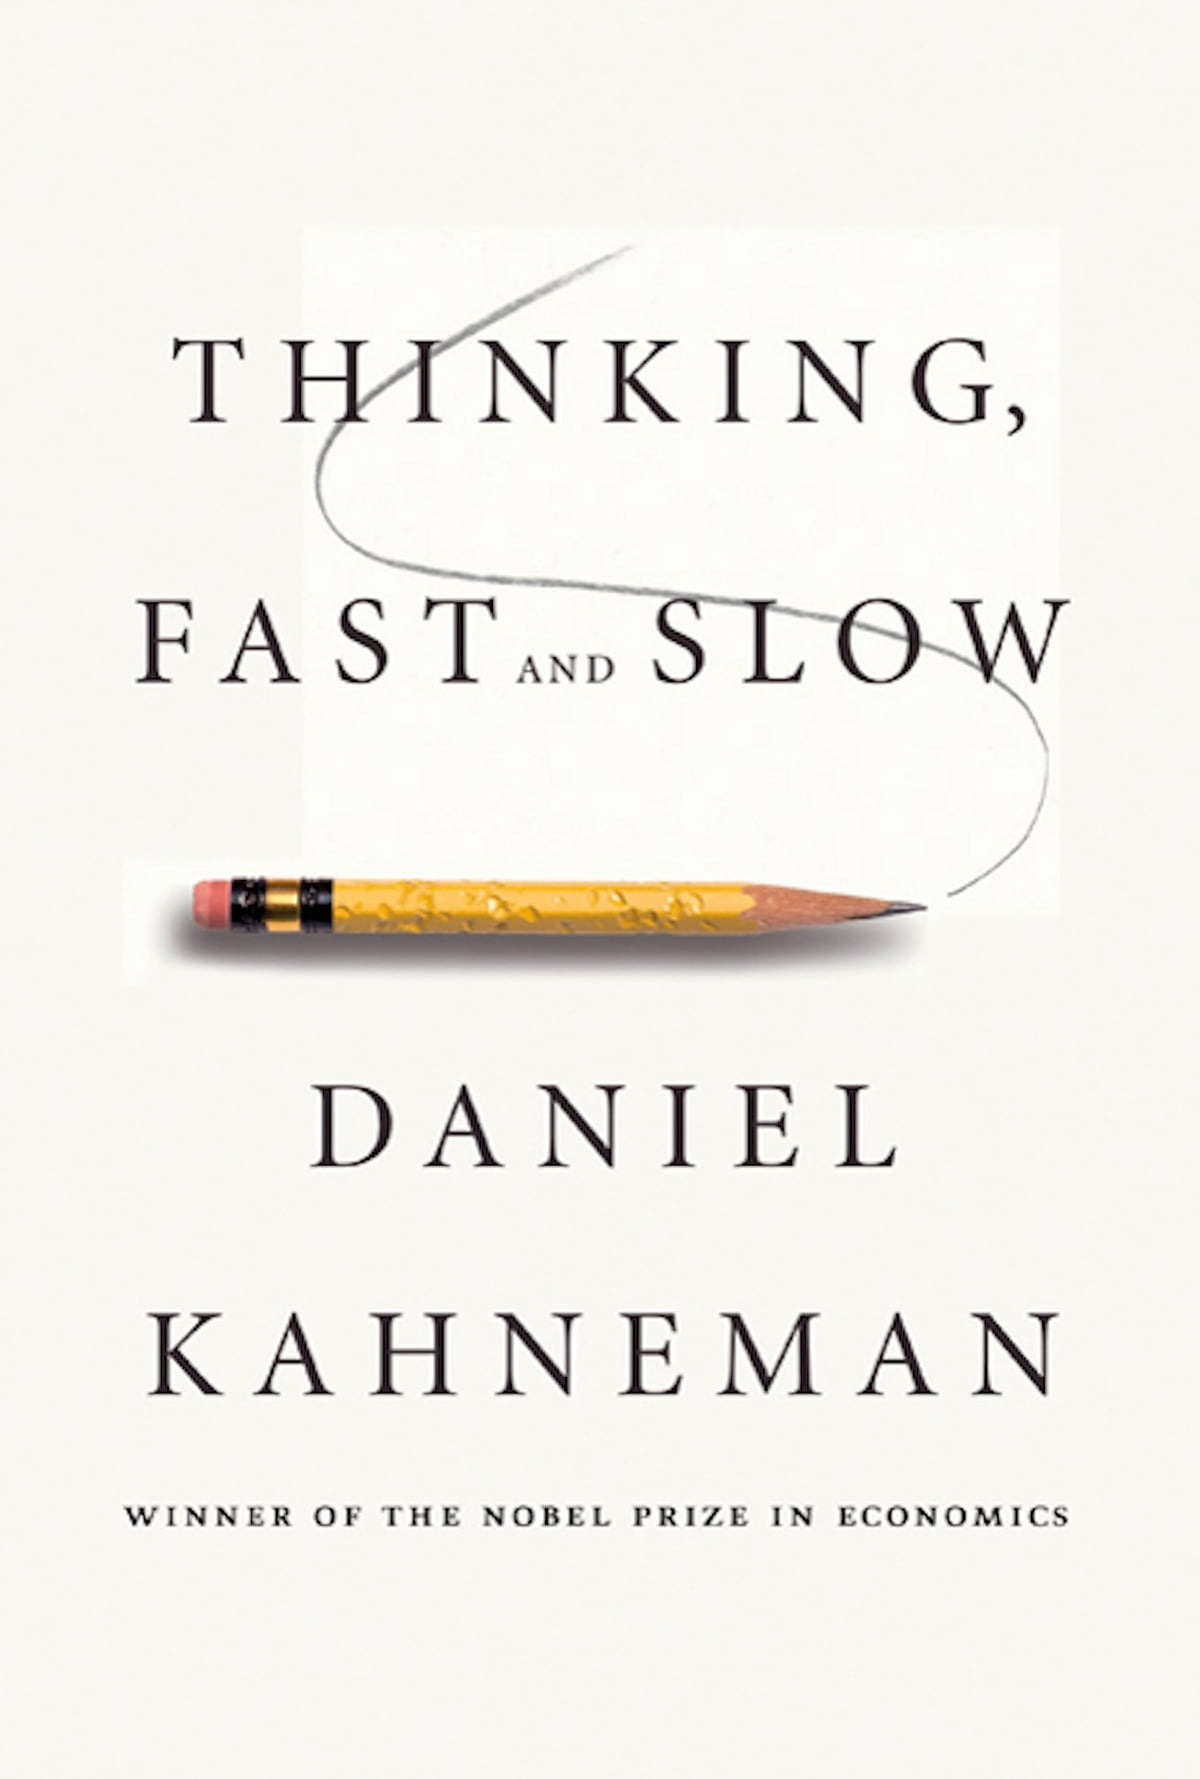
\includegraphics[width=\textwidth]{img/TFS.jpg}
        \end{minipage}
        \hspace{0.5cm}
        \begin{minipage}[t]{0.5\linewidth}
            \vspace{1cm}
            \begin{itemize}
                \item \textbf{Fast Thinking}: Correlation, pattern recognition, subconscious, ...
                \item \textbf{Slow Thinking}: Logical (causal), calculating, conscious, ...
            \end{itemize}
        \end{minipage}
    \end{figure}
    Many researchers believe that AI can only utilize "fast thinking" (System I). They propose causality to reach "slow thinking" (System II).
\end{frame}
%%%%%%%%%%%%%%%%%%%%%%%%%%%%%%%%%%%%%%%%%%%%%%%%%%%%%%%%%%%%%%%%%%%%%%%%%%%%%%%%%%%%%%%%%%%%%%%%%%%%%%%%%%%%%%%%%%%%%%%%%\begin{frame}{Reinforcement Learning}
\begin{frame}{Intuition}
\end{frame}
    